\documentclass[]{article}
\usepackage{fullpage}
\usepackage{enumerate}
\usepackage[T1,T2A]{fontenc}
\usepackage[utf8]{inputenc}
\usepackage[bulgarian]{babel}
\usepackage{soul}
\usepackage{graphicx}

\renewcommand{\thesection}{\Roman{section}} 
%\renewcommand{\thesubsection}{\thesection.\Roman{subsection}}

\begin{document}

\title{\sc{Информационна система на агенция за недвижими имоти}\\Част I: Приложение на принципите за контекстуално проектиране. Обобщен доклад.}
\author{Екип $\pi \approx 3.1$}

\maketitle

\begin{center}

\begin{tabular}{r|l}
%\hline
71469	& Георги Димов \\ %\hline
71473	& Цветан Цветанов \\ %\hline
71488	& Антон Дудов \\ %\hline
71490	& Венцислав Конов \\ %\hline
71492	& Александър Танков \\ %\hline
71508	& Красимир Тренчев \\ %\hline
71512	& Александър Велин \\ %\hline
71524	& Анджелика Туджарска \\ %\hline
71529	& Александър Бранев \\ %\hline
855240	& Мартин Стоев \\ %\hline
\end{tabular}

\end{center}

\clearpage

\tableofcontents
\clearpage

\section{Обща представа за системата} %FIXME ?
        
Трябва да се проектира информационна система за стартираща агенция за недвижими имоти, която до момента не е използвала никакви системи и няма съществуващи към момента бизнес процеси. Описаната тук система е според изискванията на собственика на агенцията.

Целта на информационната система е да осигури уеб интерфейс, чрез който брокерите могат да управляват своите обяви за недвижими имоти, а клиентите на агенцията (наематели и купувачи) да имат гъвкав и удобен интерфейс за търсене на обяви за имоти по различни критерии, както и да инициират комуникация с брокера. Връзката между собствениците на имоти и брокерите ще се осъществява извън рамките на системата.

Всички счетоводни и финансови процеси в агенцията не са предмет на информационната система.

\section{Интервюта}
В рамките на проведените интервюта бе събрана информация от следните потребители:

\begin{center}
\begin{tabular}{|l|l|}
\hline
Борислав Арнаудов & Собственик на стартираща агенция за недвижими имоти \\
\hline
\end{tabular}
\end{center}

На първото интервю (проведено на 2016-03-18 от 16:00 до 17:30 в зала 01 на ФМИ) присъстваха от страна на клиента:
\begin{itemize}
\item Борислав Арнаудов
\end{itemize}
и от страна на студентите:
\begin{itemize}
\item Георги Димов
\item Цветан Цветанов
\item Антон Дудов
\item Венцислав Конов
\item Александър Танков
\item Красимир Тренчев
\item Александър Велин
\item Анджелика Туджарска
\item Александър Бранев
\item Мартин Стоев
\end{itemize}

На второто интервю (2016-04-01 от 09:00 до 10:30 в САП България) присъстваха от страна на клиента:
\begin{itemize}
\item Борислав Арнаудов
\end{itemize}
и от страна на студентите:
\begin{itemize}
\item Георги Димов
\item Цветан Цветанов
\item Венцислав Конов
\item Александър Танков
\item Красимир Тренчев
\item Александър Велин
\item Анджелика Туджарска
\item Александър Бранев
\end{itemize}

\subsection*{Записки}
По време на интервютата бяха изяснени следните изисквания към системата:
\begin{enumerate}[I.]
\item {Функционалност на системата

% Достъп и акаунти

Системата трябва да поддържа както анонимен (публичен) достъп, така и достъп на потребители, които имат създаден акаунт в системата. Всеки акаунт има следните данни:
	\begin{itemize}
	\item username (задължителен);
	\item парола (задължителен);
	\item email (задължителен);
	\item име (задължителен);
	\item телефон;
	\item снимка.
	\end{itemize}

Брокерските профили имат натрупан до момента рейтинг на брокера.
				
Автентифицирането на потребители да се извършва от допълнителна система, свързана с основната. Данните за потребителите да се пазят на различен от основния сървър. Паролите да бъдат криптирани чрез използване на ``сол'' и силен хеширащ алгоритъм. 

% Роли
Системата трябва да поддържа следните роли:
	\begin{itemize}
	\item {нерегистриран потребител - има права да:
		\begin{itemize}
		\item търси и разглежда обяви в сайта;
		\item споделя обяви в социалните мрежи;
		\item си регистрира акаунт, с потвърждение по email, за да се гарантира вярност на вписания адрес;
		\item използва контакт формата за изпращане на съобщение към брокерите;
		\item използва чат системата, като не му се запазва log на разговора.
		\end{itemize}
	}
	\item {регистриран потребител - има права да:
		\begin{itemize}
		\item прави всички неща, които може нерегистриран потребител, освен регистрация на акаунт;
		\item използва чат системата, като се запазва log на разговора;
		\item ``запазва'' обяви, които е харесал в профила си;
		\item променя личните си данни;
		\item поиска ресет на паролата си (през email);
		\item подаде заявка, че иска да стане брокер.
		\end{itemize}
	}
	\item {брокер - има права да:
		\begin{itemize}
		\item прави всички неща, които може регистриран потребител;
		\item създава обяви за имоти;
		\item редактира и премахва своите обяви за имоти;
		\item променя състоянието на своите обяви (активни, неактивни, създадени);
		\item променя статуса на своя обява (нормална, VIP);
		\item комуникира през чат системата с други потребители, ако те са инициирали комуникацията;
		\item получава съобщения през контакт формата към дадена обява;
		\item вижда точният адрес на имота в обявите (както собствени, така и на други брокери);
		\item вижда контактната информация за собствениците на имотите в  обявите (както собствени, така и на други брокери);
		\item има право да вижда данни на даден потребител (username, email, име, телефон, снимка).
		\end{itemize}
	}
	\item {администратор (вграден в системата сервизен акаунт, единствен):
		\begin{itemize}
		\item прави всички неща, които може регистриран потребител;
		\item има право да вижда списък на потребителите в системата;
		\item има право да разглежда личните данни на потребителите (username, email, име, телефон, снимка);
		\item няма право да променя личните данни на потребителите (username, парола, email, име, телефон, снимка);
		\item има право да одобрява заявки на регистрирани потребители за промяна на статуса им към ``брокер'';
		\item има право да премахва статуса ``брокер'' от акаунти, след като е асоциирал обявите му с други брокери;
		\item има право да премахва акаунти от системата, без сервизните такива (администратор, одитор);
		\item няма право да редактира съдържанието на обява;
		\item има право да премахва обяви;
		\item има право да променя статуса на обява (нормална, VIP);
		\item има право да променя състоянието на обява (активна, неактивна) (при премахване или промяна на статуса/състоянието на обява се нотифицира брокера - собственик на обявата);
		\item има право да променя боркера-собственик на обява;
		\item получава копие от съобщенията, изпратени през контакт формата;
		\item препраща получено съобщене (от контакт форма) към брокер.
		\end{itemize}
	}
	\item одитор (вграден в системата сервизен акаунт, единствен) -- има права само да чете одит лога.
	\end{itemize}

% Обяви

Обявите се създават, редактират и премахват от брокер. Администраторът има право да редактира и премахва обявите на всички брокери.	Обявите могат да бъдат активни или неактивни, като обикновенните потребители (нерегистрирани и регистрирани) виждат само активните обяви, докато неактивните обяви са видими само за брокерите и администратора.
Обявите могат да бъдат нормални или VIP. Този статус може да се променя само ръчно от брокерите и администратора.
Обявите съдържат следните данни:
	\begin{itemize}
	\item идентификатор на брокер;
	\item натрупан до момента рейтинг на обявата;
	\item активна/неактивна обява; 
	\item нормална/VIP обява;
	\item {характеристики на имота:
		\begin{itemize}
		\item местоположение - град, квартал, улица и номер, номер на блок;
		\item детайлно местоположение - град, квартал, улица и номер, номер на блок, вход, етаж, апартамент;
		\item площ в квадратни метри;
		\item тип на цената (месечен наем/цена за закупуване), валута (BGN, USD, EUR), цена;
		\item тип на имота - апартамент, къща, гараж, парцел;
		\item {специфични характеристики според типа:
			\begin{itemize}
			\item апартамент -- тип (едностаен, двустаен, тристаен, многостаен, мезонет, студио), етаж, изложение, година и тип на строителството, прилежащи имоти (мазета, гаражи) и общи части, обзавеждане, интернет, ТЕЦ, СОТ, телефон, ток, вода;
			\item къща -- застроена и дворна площ, брой етажи, прилежащи имоти (мазета, гаражи),	обзавеждане, интернет, ТЕЦ, СОТ, телефон, ток, вода;
			\item гараж -- ток, вода;
			\item парцел -- тип (в регулация, земеделска земя), ток, вода.
			\end{itemize}
		}
		\end{itemize}
	}
	\item текстово поле -- свободно описание на обявата, до 5 KB. Полето трябва да позволява въвеждането на символи за нов ред;
	\item снимки и скици -- binary формат, до 20 броя общо, всяка с размер до 1 MB, минимум една снимка и една скица; 
	\item географски данни, описващи точната локация (GPS координати);
	\item информация за наемодателя/продавача -- имена, телефон, email, текст.
	\end{itemize}
	
Информацията за наемодателя/продавача и детайлното местоположение е достъпна само за брокерите и администратора.

% Визуализация на обява

При визуализация на детайлите на дадена обява системата трябва да:
	\begin{itemize}
	\item разграничава визуално нормалните от VIP обявите;
	\item показва контактите на брокера, свързан с обявата;
	\item предлага възможност за автоматично преизчисление на цената в алтернативна валута (BGN, USD, EUR).	Системата трябва да взима автоматично курса на БНБ;
	\item изчислява автоматично цена на квадратен метър (в текущо избраната валута);
	\item показва местоположението на обекта чрез Google Maps, на базата на GPS координатите му;
	\item преоразмерява автоматично снимките и скиците в thumbnail-и, които да показва, както и да дава възможност за разглеждане на оригиналните изображения.
	\end{itemize}
				
Ако разглеждащият обявата е брокер или администратор, системата трябва да показва и информацията за наемодателя/продавача, както и детайлното местоположение на имота.
				
Под детайлите на обявата системата трябва да предлага контактна форма за изпращане на съобщение до брокера. Формата има задължителни (име, email за обратна връзка, поле за свободен текст до 500 знака) и незадължителни (телефон за връзка) полета. Ако текущият потребител е регистриран, полетата email и телефон се попълват автоматично от системата с тези от профила на потребителя, като системата осигурява възможност на потребителя да ги редактира преди изпращане на съобщението. Изпращането на съобщения е еднопосочно - от потребители към брокер, и няма възможност за отговор през системата. Копие от всички изпратени през формата за контакт съобщения се изпраща до администратора.

% Система за търсене

Потребителите да могат да търсят обяви в системата по зададени критерии за търсене. Критериите се задават на етапи.
\begin{enumerate}[a) ]
\item Избор на населено място. Потребителят да може да избира населено място от списък  или, ако не е на мобилно устройство, от карта на страната. 
\item Квартал / район. От списък с районите за съответното населено място потребителят може да избира специфичен район, в който да търси обяви. Ако не е на мобилно устройство, може също да избира район карта на населеното място, което е избрал.
\item Избор на допълнителни параметри. Включват се всички характеристични полета с краен брой стойности. Потребителя да може да избира повече от едно поле.
\end{enumerate}

Да се предостави възможност за търсене по текст от полетата на обявите. Потребителят да може да въвежда свободен текст в поле за търсене. Търсенето се осъществява по всички видими за потребителя текстови полета на обявата (вкл. адрес, свободен текст към обявата и т.н.). Да се предостави възможност за връщане назад по стъпките и промяна на критериите и филтрите за търсене.

\emph{Заб. Някои от полетата за търсене са приложими само за някои от типовете имоти.}

В резултата от търсенето да се изобрази списък от обяви, които отговарят на максимален брой полета от критериите и филтрите за търсене, които потребителят е задал. Ако в резултатите има VIP обяви, то те да се показват с приоритет (преди останалите обяви), като се различават от останалите визуално. Няма ограничение за броя VIP обяви на страница.

%FIXME Чат

%Системата трябва да предоставя функционалност на нерегистрираните и регистрираните потребители да провеждат текстова комуникация в реално време с брокер. Потребителите могат да задават въпроси в чата, а брокерите, които са на работа наблюдават въпросите и отговарят на тях, като комуникацията е двустранна. Брокерите виждат само имената и въпросите на потребителите. Анонимните потребители трябва да предоставят име, което да използват в чата. Системата трябва да запазва историята на чат сесиите на регистираните потребители, и да им предоставя възможност да я разглеждат.
%----------

Чат системата дава възможност на потребителите да се свържат в реално време с брокер от агенцията. Комуникацията става посредством обмяна на текстови съобщения между двете страни. 

Потребителите виждат бутон за чат в системата, както и означение за това дали в момента има брокери на линия. Инициирането на чат сесия се извършва от потребителя с първото изпратено съобщение. В този момент за потребителя се създава виртуална чат стая, която е активна докато потребителя е на линия (в системата).

Брокерите виждат всички чат стаи, статусите им и изпратените съобщения в стаята чрез специален интерфейс в системата. Също имат възможност да се присъединят към коя да е чат стая. 

В една чат стая присъства само един потребител, но е възможно да присъстват множество брокери. От гледна точка на потребителя има само един брокер -- съобщенията от няколко брокера се визуализират идентично.

Статуса на чат стаята може да бъде:
\begin{itemize}
\item неактивна -- означава, че потребителят е затворил чата си или е излязъл от системата;
\item непрочетена -- означава, че съобщенията, изпратени от потребителя все още не са били прочетени от никой брокер;
\item прочетена -- означава, че съобщенията са прочетени.
\end{itemize}

Чат системата може да се използва както от регистрирани, така и от нерегистрирани потребители. За име в чата на регистрираните потребители се използва името от профила на потребителя, а за нерегистрираните се изисква въвеждане на име при започване на чата. Регистрираните потребители също така имат възможност да виждат хронология на предишните си чатове - тя се запазва в профила им.

Чатът не е обвързан с обявите в системата или с брокерите - всеки брокер може да отговаря на всеки потребител.

% Одит лог

Системата трябва да поддържа одит лог, в който да записва всички действия на регистрирани потребители във системата. Логовете съдържат:
	\begin{itemize}
	\item дата и час на събитието;
	\item извършител (username);
	\item от къде е извършено действието (IP адрес);
	\item тип на действието;
	\item субект на действието;
	\item старата и новата стойност на промененото поле, ако е парола -- звездички.
	\end{itemize}
Записват се всички промени върху потребителските профили и обявите, както и изпратените съобщения от контакт формата.
Одит лога може да се чете само от одиторския акаунт и не може да се променя от никого. Събитията, по-стари от 6 месеца, се премахват от лога.

% Рейтингова система за брокерите и обявите

Всяка обява има собствен рейтинг по скалата от 0 до 5. Визуализира се заедно с обявата под формата на пет звезди, като част от тях са запълнени, съответно показващи текущия рейтинг на обявата. Потребителите имат право да гласуват за обяви с оценки от 1 до 5. Изчислява се среден рейтинг на обявата спрямо събраната сума от всички гласувания, разделена на броя гласували. Рейтингът на дадена обява не участва по никакъв начин в търсенето или сортирането на обяви, той служи само за визуализация. 

Брокерите също имат рейтинг, подобен на този на обявите. Потребителите могат да гласуват за брокер независимо от обявите му, както и могат да гласуват за обяви независимо от брокера. Няма връзка между рейтингите на обява и на брокера, който я е пуснал. 

Брокерите и обявите започват с рейтинг 0, което означава, че никой не е гласувал за тях. 


} %Функционалност на системата

\item {Нефункционални изисквания
	
Системата трябва да:
	\begin{itemize}
	\item е достъпна през уеб интерфейс;
	\item поддържа около 100-150 посещения на ден;
	\item поддържа 1000 регистрирани потребителя;
	\item поддържа 400 активни обяви;
	\item поддържа 10000 обяви общо (активни и неактивни);
	\item осигурява резултат при търсене до 3 секунди;
	\item осигурява зареждане на страница за до 1-1.5 секунди;
	\item поддържа паролите в криптиран вид;
	\item може да работи върху GNU/Linux операционна система;
	\item може да е в експлоатация 10 години;
	\item има автоматичен онлайн бекъп не по-рядко от веднъж на 24 часа;
	\item потребителските сесии в системата изтичат автоматично при 1 час неактивност на потребителя.
	\end{itemize}
		
Допустимият downtime на системата е не повече от 48 часа общо на година.
} %Нефункционални изисквания

\item {Интеграция с външни системи

Системата трябва да предлага възможност на потребителите (регистирани и нерегистрирани) да споделят дадена обява в социалните мрежи (Facebook, Twitter, Google+).

Системата трябва да може да показва местоположението на даден имот в Google Maps на базата на GPS координатите в обявата.

Системата трябва да поддържа възможност за Google Ads.

Системата трябва да може автоматично да взима валутните курсове (BGN/USD/EUR) от БНБ.	
} %Интеграция с външни системи

\end{enumerate}

\section{Модели}

\subsection*{Contextual Design - flow модели}
На базата на събраната информация бяха идентифицирани следните роли:
\begin{itemize}
	\item нерегистриран потребител;
	\item регистриран потребител;
	\item брокер;
	\item администратор;
	\item одитор.
\end{itemize}
За всяка роля беше проучен и описан съответстващият ѝ модел на дейностите.

\begin{enumerate}[I.]
	\item {Модел на дейностите на Нерегистриран потребител
	
\emph{Моделът е показан на Фигура 1.} 

Оглед на дейности и отговорности на нерегистрирания потребител:
	
		\begin{itemize}
		\item {Търсене на обяви – Потребителят използва търсачка, чрез която въвежда своите изисквания за имоти. Направената заявка се изпраща до пълният каталог от активни обяви. Каталогът връща списък с обяви, които отговарят на изискванията на потребителя.
}
		\item {Споделяне на обяви – Потребителят може да споделя обяви в социалните мрежи.
}

		\item {Връзка с брокер през контакт форма – Потребителят се намира в конкретна обява и изявява желанието да се свърже с брокер за повече информация. Попълва контакт форма за съответната обява като трябва да въведе името си, email и не повече от 500 символа в полето за свободен текст. Има възможност да остави телефон за връзка в предназначеното поле. Контакт формата се препраща както до брокера, така и до администратора. При отсъсващ брокер, администраторът препраща обявата до друг брокер.
}
		\item {Използване на чат – Потребителят иска да получи обща информация. За целта има възможността да ползва чат системата на сайта, когато тя е активна. Системата е активна, когато има брокери, които са на разположение. Потребителят, когато изпраща съобщение чрез чат системата трябва да въведе името си. Съобщението се препраща под формата на известие на брокерите, които са на линия. Потребителят получава известие за непрочетено съобщение, когато брокер отговори на негово съобщението.
}
		\item {Регистрира се – Потребителят за да се регистрира трябва да попълни задължителните полета (username, име, email, парола) на регистрационната форма зад бутона Sing in. При попълнени полета username и email системата се грижи да провери дали вече съществуват в списък с регистрирани потребители. При съвпадение на тези полета потребителят получава известие и трябва да ги смени. Потребителят може да добави снимка и телефон по желание. Като снимката трябва да е не повече от 1 MB. След успешно попълнена регистрационна форма системата изпраща потвърждаваш регистрацията email до посочения от потребителя email-адрес. Потребителят потвърждава регистрацията си и системата изписва съобщения за успешно направена регистрация.
}
		\end{itemize}
		
	\begin{figure}[h]
	\centering
	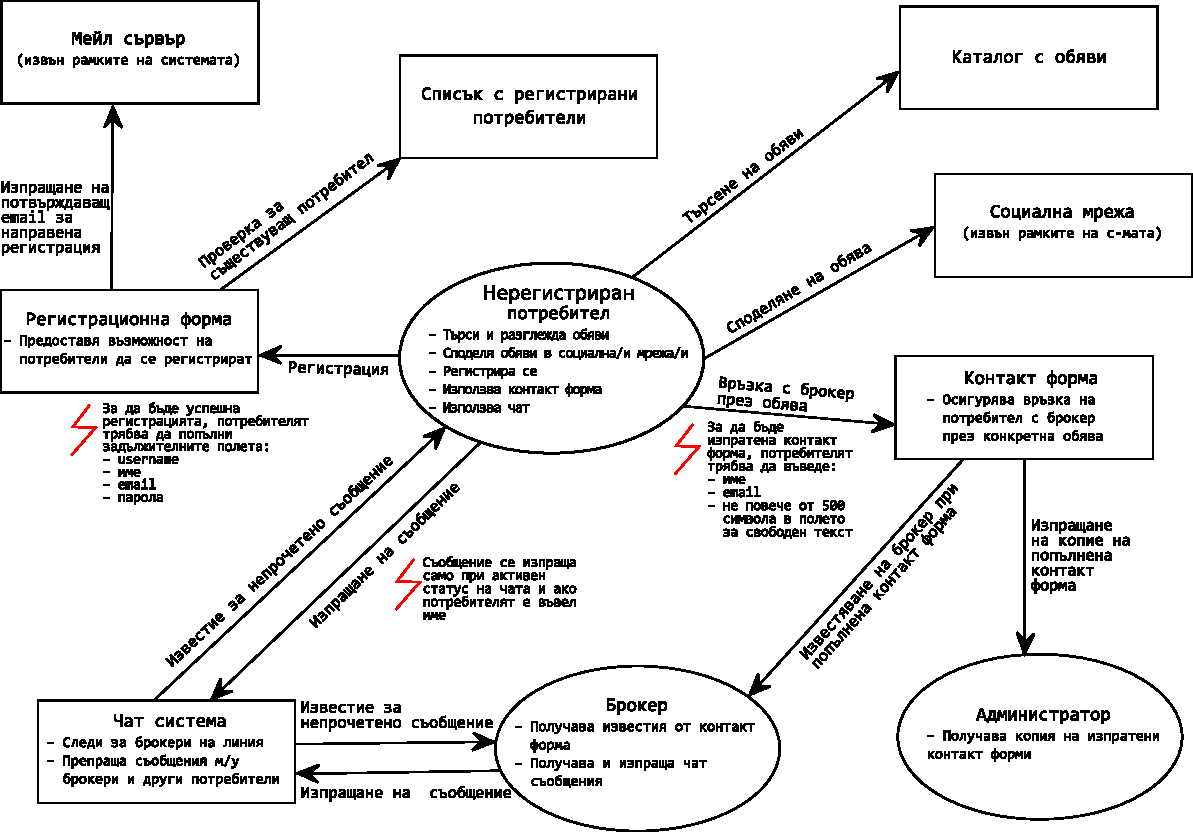
\includegraphics[scale=0.75]{flow-unregistered-user}
	\caption{Flow модел за Нерегистриран потребител}
	\end{figure}

	} % нерегистриран
	
% FIXME	
	\item {Модел на дейностите на Регистриран потребител

\emph{Моделът е показан на Фигура 2.} 

Ролята има същите възможности които има и нерегистрираният потребител, но му се пази история на чат сесиите, и може да запазва обява към профила си.

	\begin{figure}[h]
	\centering
	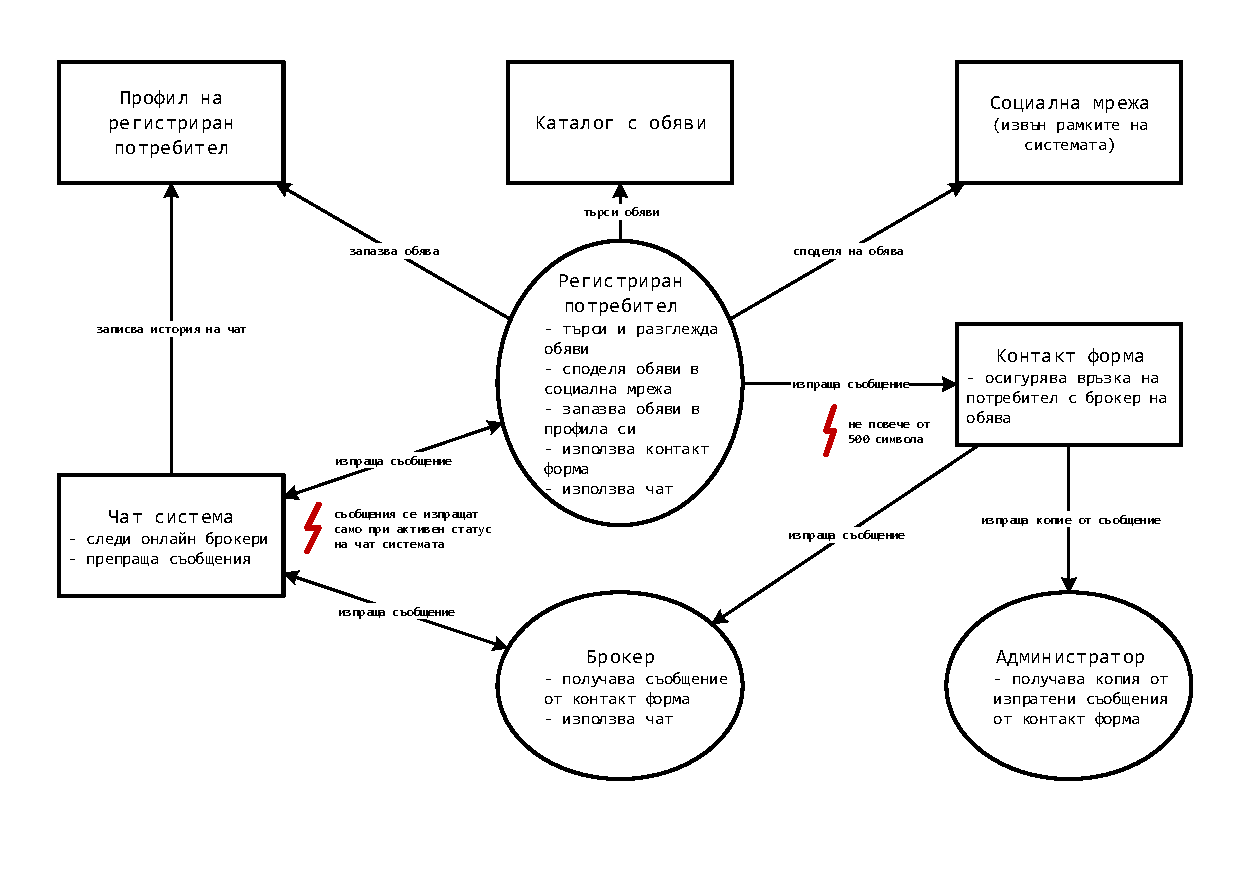
\includegraphics[scale=0.85]{a1-flow-reg}
	\caption{Flow модел за Регистриран потребител}
	\end{figure}

	} % регистриран	
	
	\item {Модел на дейностите на Брокер

\emph{Моделът е показан на Фигура 3.} 

Този модел показва дейностите, които извършва и за които е отговорен един брокер в системата. В тях се включват всички дейности, които може да извършва регистрираният потребител, като в допълнение основната дейност на брокера е да създава и редактира обяви в системата. Комуникацията му със собствениците или наемодателите на имоти е ключова за създаването на обяви, но не влиза в областта на действие на системата.
 
Всяка обява задължително трябва да има поне една снимка и задължение на брокера е да заснеме снимки и да редактира обявата, като ги добавя в нея.

Отговарянето на контакт форма също е задължение на брокера, което се извършва по методи, външни за системата (най-често e-mail). 

Комуникацията, която протича през системата за чат в работно време е двустранна, като се инициира от потребители. По този начин се създават виртуални чат стаи и неограничен брой брокери могат да отговарят на съобщения от даден потребител. Чат системата следи също и за наличието на брокери онлайн и уведомява потребителите. 

	\begin{figure}[h]
	\centering
	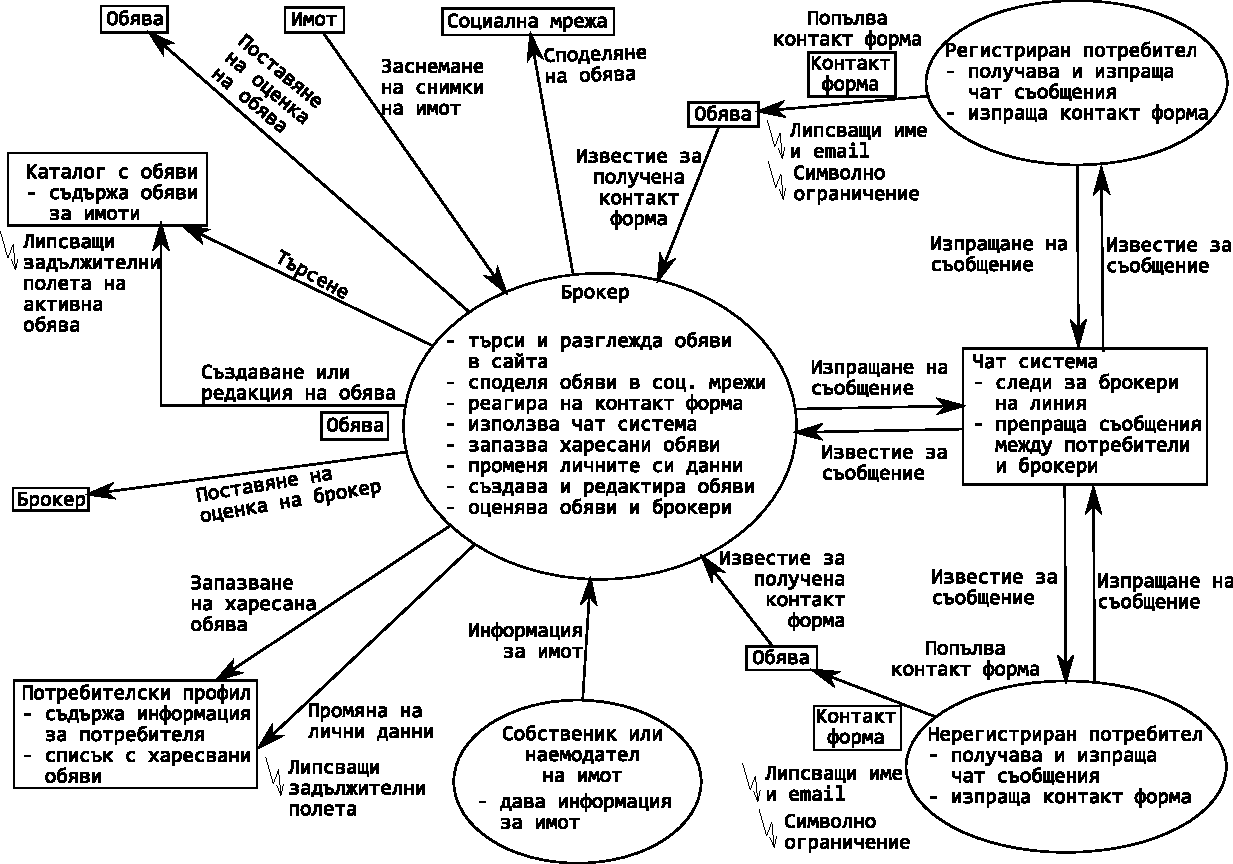
\includegraphics[scale=0.85]{flow-broker}
	\caption{Flow модел за Брокер}
	\end{figure}
	
	} % брокер

	\item {Модел на дейностите на Администратор

\emph{Моделът е показан на Фигура 4.} 

Съществува един администраторски акаунт, който е вграден в системата, т.е. не се създава допълнително, а го получаваме наготово. Той има всички функционалности, които притежават регистрираните и нерегистрираните потребители - може да разглежда, търси, харесва, споделя в социалните мрежи обяви. Може да използва чат системата и да изпраща съобщения чрез контактната форма. Тези неща умишлено са пропуснати в диаграмата, понеже не са съществени към цялостната работа на ролята.

Основните дейности на администратора се изразяват в редактиране на обяви, като под това се има предвид смяна на статуса между нормална и вип обява, промяна на състоянието и между публикувана и непубликувана. Също така може да изтрива обяви от системата или да променя принадлежността им към конкретен брокер. Други дейности са редактиране на потребителски профил, като тук се има предвид одобряване или отхвърляне на заявка от даден потребител, изразяваща желанието му да стане брокер. Това се определя на базата на хартиен списък, предоставен от мениджъра на фирмата. Може също да променя брокерските профили обратно към потребителски или да ги изтрива. При това действие е задължен да асоциира обявите да въпросния брокер към някой друг.

Администраторът получава копие от всяко съобщение, което потребителите са изпратили през контактната форма и има възможността да го препрати към избран от него брокер.

	\begin{figure}[h]
	\centering
	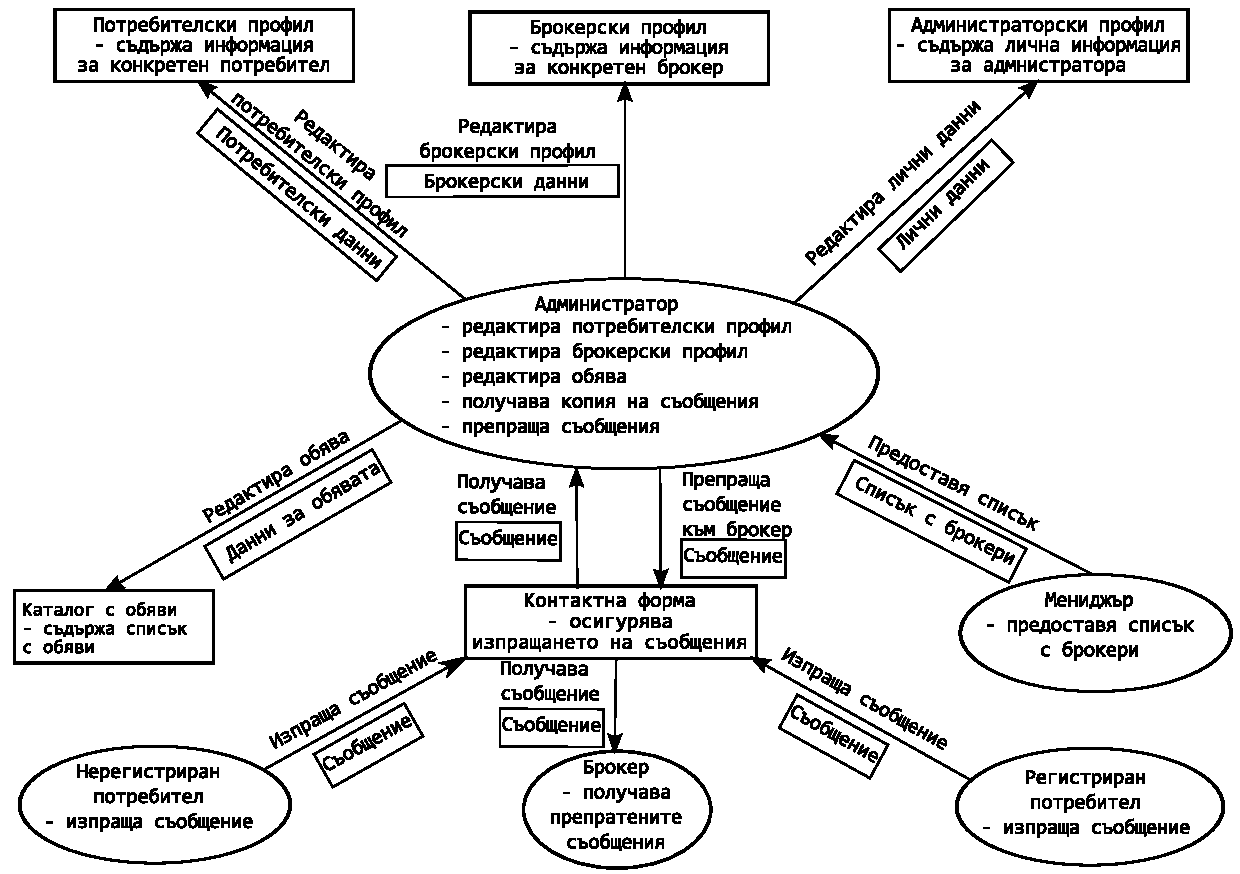
\includegraphics[scale=0.85]{flow-administrator}
	\caption{Flow модел за Администратор}
	\end{figure}
	
	} % админ
	
	\item {Модел на дейностите на Одитор

\emph{Моделът е показан на Фигура 5.} 

В системата съсществува вграден акаунт за одитор, който има права само да чете одит лога. При нужда от информация за настъпила промяна в системата (за даден акаунт, обява и т.н.), брокерите, администраторът, собственикът на фирмата могат да поискат от одитора информация защо е настъпила промяната. 
	
\emph{Заб. Одиторът може да откаже достъп до поисканата информация. Правилата за допуск са извън обхвата на системата.}

	\begin{figure}[h]
	\centering
	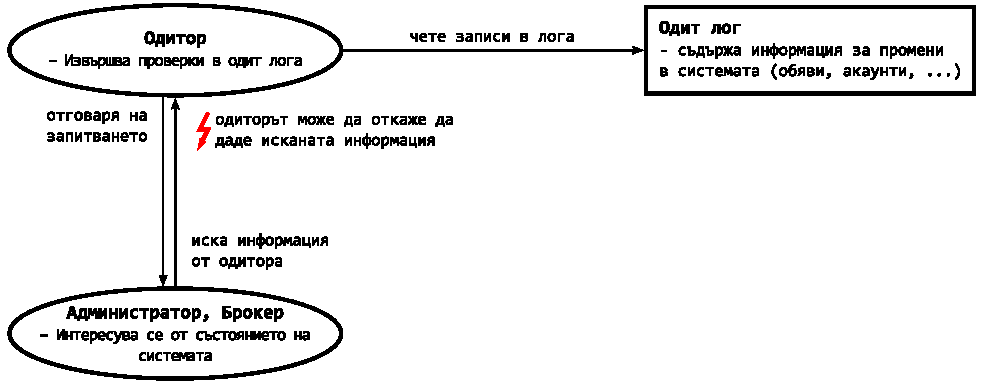
\includegraphics[scale=0.85]{flow-auditor-small}
	\caption{Flow модел за Одитор}
	\end{figure}
	
	} % одитор	
	
\end{enumerate}

\clearpage

\subsection*{Contextual Design - sequence модели}

На базата на събраната информация бяха идентифицирани по-важни последователности:
\begin{itemize}
	\item търсене на обява;
	\item регистриране на потребител;
	\item брокер добавя имот;
	\item потребител изпраща съобщение чрез контакт форма;
	\item процедура за промяна на парола;
	\item администратор променя статус брокер на акаунт;
	\item администратор препраща получени съобщения от контакт фромата.
\end{itemize}
Първите три (търсене на обява, регистриране на потребител, добавяне на имот от брокер), като основни, бяха проучени и моделирани.

\begin{enumerate}[I.]

	\item {Модел на последователностите при търсене на обява
	
Този модел включва последователното отсяване на обяви чрез критерии за търсене, като се започва от най-високия -- търсене по град, до най-финия -- търсене по ключови думи. На всеки етап на потебителя е предоставена възможността да се върне назад и да промени критериите си за търсене. Само при изцяло попълнени критерии на потребителя се предоставя окончателният списък с обяви.

\begin{center}
  \begin{tabular}{ |p{6cm}|p{10cm}| }
    \hline
    \multicolumn{2}{|c|}{\textbf{Намерение}: Потребител желае да потърси обяви по даден критерий.} \\    \hline
    & \textbf{Тригер}: Потребител натиска бутон ``Търси''. \\    \hline
    \textbf{Намерение}: Да се намери обява в регион, удобен за потребителя. & Появява се списък с населени места, ако е на мобилно устройство, иначе се появява карта на страната. \\    \hline
    \textbf{Бележка}: Потребителят може да се върне назад за да поправи критерия. & \\    \hline
      & Потребителят се препраща към стъпка за избиране на квартал/район. \\    \hline
    \textbf{Намерение}: Да се намери обява в квартал/район, удобен за потребителя. & Появява се карта на текущо избраното населено място, от която потребителят може да избира квартал/район. Ако е на мобилно устройство се появява само списък. \\    \hline
    \textbf{Бележка}: Потребителят може да се върне назад за да поправи критерия. & \\    \hline
     & Потребителят се препраща към стъпка за избиране на характеристики на имота. \\    \hline
    \textbf{Намерение}: Да се избере имот, който спазва нужните на потребителя характеристики. & Появяват се полета с характеристики, от които потребителят може да избира. Валидно е да се избере повече от една характеристика. \\    \hline
    \textbf{Бележка}: Потребителят може да се върне назад за да поправи критерия. & \\    \hline
     & Предоставя се поле за търсене. \\    \hline
    \textbf{Намерение}: Филтриране на получените резултати чрез търсене в текстовите полета на обявите. & Предоставя се поле за търсене, където потребителят въвежда свободен текст. По този свободен текст се филтрират тези обяви, които го имат в полетата си. \\    \hline
    \textbf{Бележка}: Потребителят може да се върне назад за да поправи критерия. & \\    \hline
    \textbf{Намерение}: Уведомяване на потребителя за наличните обяви. & Повявява се списък с обявите спазващи горните четири критерия. \\    \hline
  \end{tabular}
\end{center}

	
	} % search
	
	\item {Модел на последователностите при регистриране на потребител
	
Този модел на последователностите представя действията на потребител по време на създаването на акаунт. Той включва последователното попълване на личните данни от потребителя, при което, ако има грешка, той бива върнат да попълни данните правилно. Само когато всичко е попълнено коректно, тогава на потребителя се изпраща email с временен линк за потвърждение на регистрацията. При успешно потвърждение акаунтът се създава в системата, като автентифициращата информация се запазва в система, различна от основната.

\begin{center}
  \begin{tabular}{ |p{5cm}|p{10cm}| }
    \hline
    \multicolumn{2}{|c|}{\textbf{Намерение}: Нерегистриран потребител желае да се регистрира} \\
    \hline
    & \textbf{Тригер}: Потребил натиска бутон ``регистрация''. \\
    \hline
      \textbf{Намерение}: Потребителят попълва данните & Показва се форма за попълване на личните данни на потребителя. \\
    \hline
     & След попълването се изчаква потребителя за натискане на бутон ``регистрирай ме''. \\
    \hline
    \textbf{Намерение}: Проверка на данните, въведени от потребителя. & Потребителското име се проверява за уникалност. \\
    \hline
     & Паролите, въведени от потребителя, се проверяват спрямо критериите за сигурност. \\
    \hline
     & Проверка за валидност на email адреса. \\
    \hline
     & Името се проверява дали съдържа само букви. \\
    \hline
    \textbf{Бележка}: Потребителя се уведомява за грешка, ако такава съществува.  & \\
    \hline
      & Потребителят се препраща към полето, в което има грешка, ако са повече от една се препраща към първото поле. \\
    \hline
    \textbf{Намерение}: Добавяне на номер на телефон и снимка. & Ако потребителят е осигурил номер на телефон и снимка, те се добавят в потребителския акаунт.  \\
    \hline
    \textbf{Намерение}:  Верификация на вече създадения потребителски акаунт. & Изпраща се email до адреса, въведен от потребителя.  \\
    \hline
     & След изпращането се изчаква за потвърждаване от страна на потребителя. \\
    \hline
    \textbf{Намерение}: Съхранение на паролата на потребителя. & Изчаква се обработката и запазването на потребителската парола от страна на външната система\\
    \hline
    \textbf{Намерение}: Уведомяване на потребителя за успешно регистриране. & Потребителят бива препратен към страницата за вход. \\
    \hline
  \end{tabular}
\end{center}

	
	} % регистриране	
	
	\item {Модел на последователностите при добавяне на обява от брокер

Този модел на последователностите представя действията на брокер по време на създаване на обявa. Той включва последователното попълване на данните на една обява, при което, ако има полета за данни, които са задължителни и не са попълнени, брокерът бива върнат, за да ги попълни.

Само когато всички задължителни полета са попълнени, тогава на брокера се дава възможност да създаде обявата.

\begin{center}
  \begin{tabular}{ |p{5cm}|p{10cm}| }
    \hline
    \multicolumn{2}{|c|}{\textbf{Намерение}: Брокер желае да създаде обява} \\
    \hline
    	& \textbf{Тригер}: Брокерът натиска бутон ``Създаване на обява''. \\
    \hline
    	\textbf{Намерение}: Брокерът попълва данните & След попълването на полетата на обявата се изчаква натискане на бутон ``Създай обявата''  \\  
	\hline
    	\textbf{Намерение}: Проверка на данните въведени от брокера & Проверява се обявата има ли снимка \\
    \hline
    	& Проверява се обявата има ли скица \\
    \hline
    	& Проверява се обявата има ли цена \\
    \hline
    	& Проверява се обявата има ли обявено място на имота \\
    \hline
        \textbf{Бележка}: Брокерът се уведомява за грешка, ако не е попълнено някое задължително поле & \\
    \hline     
    	& Брокерът се препраща към полето, което не е попълнено. Ако са повече от едно, се препраща към първото. \\
    \hline
    	\textbf{Намерение}: Уведомяване за успешно създаване на обява & \\
    \hline
  \end{tabular}
\end{center}
	
	} % добавяне на обява	
	
\end{enumerate}

\subsection*{Contextual Design - artifact модели}

На базата на събраната информация бяха идентифицирани следните по-важни артефакти:
\begin{itemize}
	\item данни за определена обява - адрес, цена, характеристични полета, снимки и т.н.;
	\item списък с всички брокери на агенцията (на хартия);
	\item съобщение, изпратено през контактната форма;
	\item набор от критерии за търсене;
	\item акаунт (профил) в системата.
\end{itemize}

Първите два (данни на обява, списък с брокери) бяха моделирани.

\begin{enumerate}[I.]
	\item {Модел на данни на обява
		
		\emph{Моделът е показан на Фигура 6.} 
		
		Пояснения към полетата в модела:
		\begin{itemize}
		\item жизненият статус на обявата може да бъде Активен или Неактивен, като съответно се вижда или не от потребителите;
		\item преференциалният статус може да бъде VIP обява или Обикновенна обява, като VIP обявите се показват първи при търсене;
		\item вход, етаж и апартамент са видими само за ролите администратор и брокер;
		\item GPS координати - точна локация, изобразява се чрез Google Maps;
		\item снимките и скиците - поне една снимка и една скица, като общо да са най-много 20, всяка с размер до 1MB;
		\item свободният текст да е най-много 5000 знака.
		\end{itemize}

	\begin{figure}[h]
	\centering
	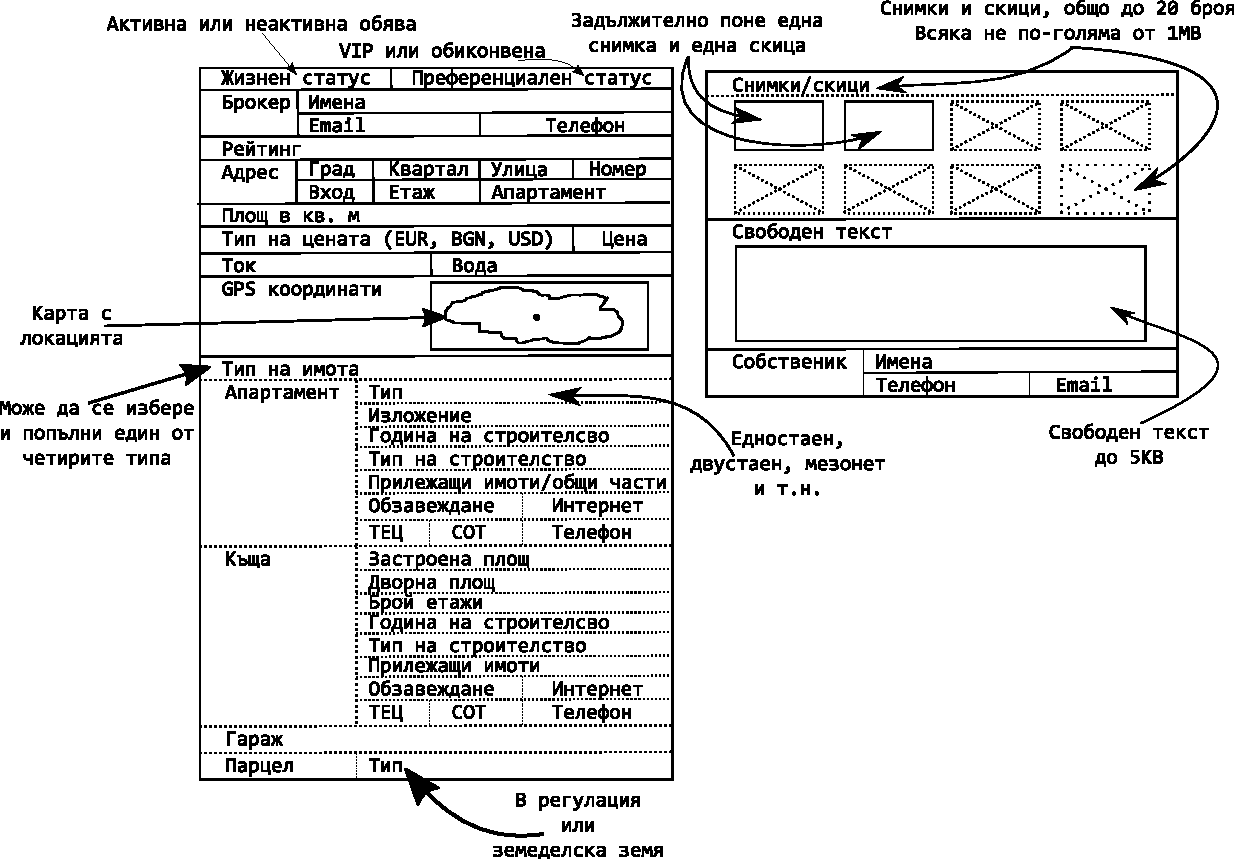
\includegraphics[scale=0.85]{art-offer}
	\caption{Artifact модел за Данни на обява}
	\end{figure}
	
	}
	
	\item {Модел на списък с брокери

Артефактът \emph{(моделът е показан на Фигура 7.)} представлява списък (на хартия) с всички брокери на агенцията, който мениджърът предоставя на администратора. Разделен е на 3 основни части:
	\begin{itemize}
	\item Заглавна част, в която се записва информация за природата на документа.
	\item {Тяло, което се дели на 2 части:
		\begin{itemize}
		\item {Описание на полета на следващите редове. Дели са на 4 части (от ляво на дясно):
			\begin{itemize}
			\item Номер - Номер на записа;
			\item Три имена - Съдържа 3-те имена на одобрените брокери;
			\item Email - Съдържа email адрес на одобрения брокер;
			\item Дата на наемане - Съдържа датата, на която брокера е бил нает.
			\end{itemize}					
		}
		\item Съвкупност от записи, имащи гореописания формат.
		\end{itemize}
		}
	\item Заключителна част (Footer) - съдържа номер на страницата.
	\end{itemize}		

Име и email адрес са полетата, по които администраторът идентифицира наетите от фирмата брокери. Ако акаунт, поискал повишение в брокер, не притежава характеристики, идентични с описаните в документа, то администраторът отхвърля искането. Ако характеристиките съвпадат, администраторът повишава акаунта в брокер. При нужда от добавяне на описание на нови брокери, артефактът минава в притежание на мениджъра, докато бъде попълнен, след което се връща отново при администратора. 

	\begin{figure}[h]
	\centering
	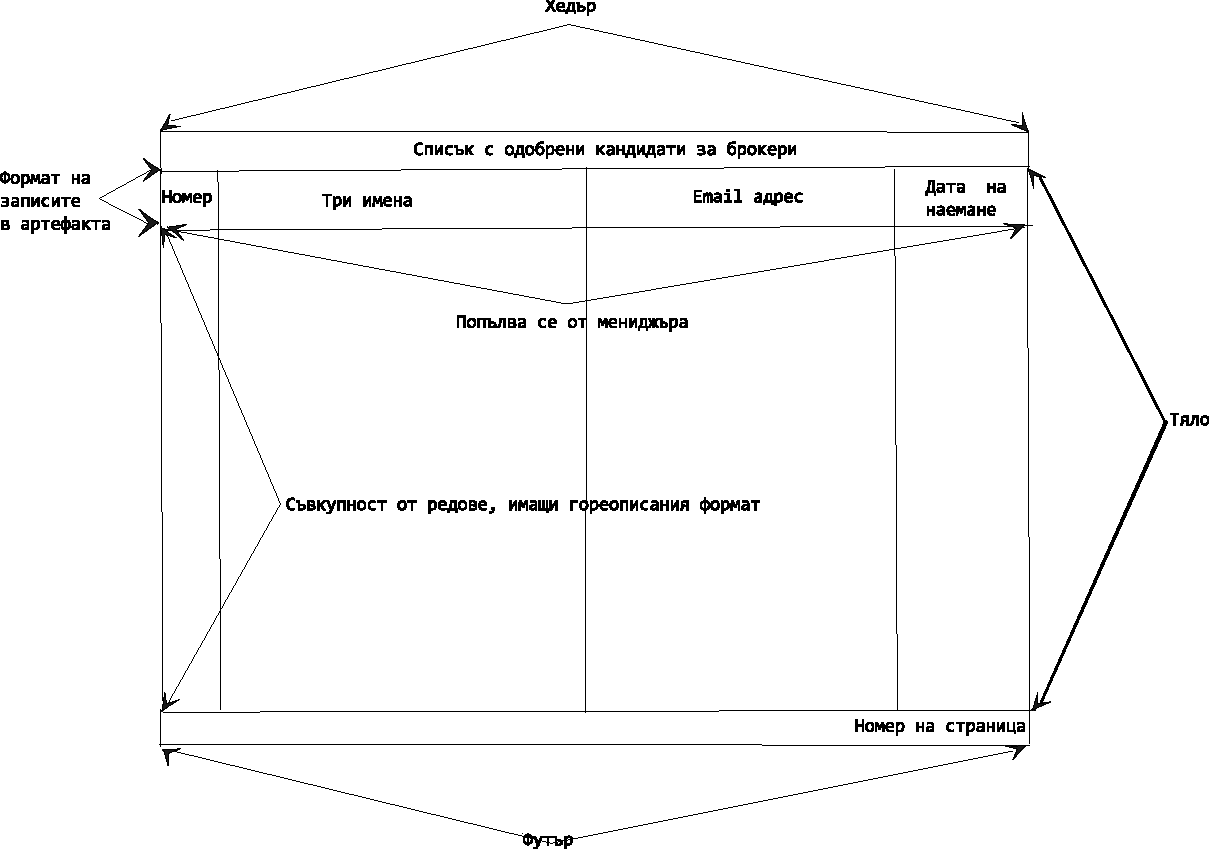
\includegraphics[scale=0.85]{art-textFile}
	\caption{Artifact модел за Списък с брокери}
	\end{figure}

	
	}
	
\end{enumerate}

\clearpage

\section{Разпределение на времето и задачи}

\begin{table}[h]
\centering
\caption{Време в минути за работа на всеки студент в различните етапи}
\label{my-label}
\begin{tabular}{|l|l|l|l|l|l|l|l|l|l|l|}
\hline
                        & 71469 & 71473 & 71488 & 71490 & 71492 & 71508 & 71512 & 71524 & 71529 & 855240 \\ \hline
Интервю 1               & 90    & 90    & 90    & 90    & 90    & 90    & 90    & 90    & 90    & 90     \\ \hline
Интервю 2               & 90    & 90    & 0     & 90    & 90    & 90    & 90    & 90    & 90    & 0      \\ \hline
Транскрибиране 1        & 140   & 45    & 90    & 140   & 150   & 90    & 90    & 150   & 150   & 120    \\ \hline
Транскрибиране 2        & 100   & 30    & 90    & 75    & 120   & 60    & 120   & 150   & 90    & 60     \\ \hline
Записки 1               & 60    & 30    & 60    & 60    & 30    & 60    & 0     & 180   & 60    & 30     \\ \hline
Записки 2               &       & 15    &       & 45    & 30    & 20    & 0     & 10    & 0     & 0      \\ \hline
Резюме 1                & 90    & 0     & 90    & 70    & 90    & 60    & 360   & 60    & 60    & 50     \\ \hline
Резюме 2                & 10    & 0     &       & 80    & 0     &       & 120   & 60    & 0     & 0      \\ \hline
Уточняване на модели    & 60    & 120   &       & 80    & 30    & 120   & 60    & 120   & 0     &        \\ \hline
Работа по CD модели     & 350   & 60    & 300   & 180   & 120   & 390   & 120   & 180   & 0     &        \\ \hline
Подготовка на доклад 1  & 0     & 0     &       & 50    & 0     &       & 540   &       & 0     &        \\ \hline
\textbf{Общо}           & 990   & 480   & 720   & 960   & 750   & 980   & 1590  & 1090  & 540   & 350    \\ \hline
\end{tabular}
\end{table}

\begin{table}[h]
\centering
\caption{Разпределение на работата по моделите}
\label{my-label}
\begin{tabular}{|l|l|l|}
\hline
\textbf{ф.н.} & \textbf{Име}        & \textbf{Модел}                                               \\ \hline
71469         & Георги Димов        & Модел на дейностите на Администратор                         \\ \hline
71473         & Цветан Цветанов     & Модел на последователностите при търсене на обява            \\ \hline
71488         & Антон Дудов         & Модел на данни на обява                                      \\ \hline
71490         & Венцислав Конов     & Модел на дейностите на Брокер                                \\ \hline
71492         & Александър Танков   & Модел на последователностите при добавяне на обява от брокер \\ \hline
71508         & Красимир Тренчев    & Модел на списък с брокери                                    \\ \hline
71512         & Александър Велин    & Модел на дейностите на Одитор                                \\ \hline
71524         & Анджелика Туджарска & Модел на дейностите на Нерегистриран потребител              \\ \hline
71529         & Александър Бранев   & \textit{Модел на дейностите на Регистриран потребител}       \\ \hline
855240        & Мартин Стоев        & Модел на последователностите при регистриране на потребител  \\ \hline
\end{tabular}
\end{table}

\end{document}
